% !TEX root=../main.tex

\section{Attention and Anticipation}\label{sec:anticipation}

The attention and anticipation algorithm~\cite{Carlone2017} selects a subset $\mathsf{S}$ of the features $\mathsf{F}$ detected in the current frame to pass to the VIO back end.
The subset of features should have at most $\kappa$ features that are the most useful (as a set) for reducing uncertainty in vision-based state estimation.
This feature selection problem can be stated as
\begin{equation}\label{eqn:sensor-selection-problem}
\max_{\mathsf{S}\subset\mathsf{F}} \quad f(\mathsf{S}) \qquad \text{subject to}\quad |\mathsf{S}|\le\kappa.
\end{equation}
The solution of this problem relies on the selection of a metric $f$ that maps subsets of features to their usefulness.

Although sensor selection problems have been shown to be NP-hard because of the introduction of binary selection variables, recent results have leveraged submodular cost functions to allow greedy algorithms to efficiently find solutions to Problem~\eqref{eqn:sensor-selection-problem} with guarantees on suboptimality~\cite{Shamaiah2010}.
% \pcl{define what a submodular set function is.}
The goal then is to identify a performance metric that exhibits submodularity and captures the accuracy of VIO.

Following~\cite{Carlone2017}, we use the logdet metric to measure the volume of the estimation uncertainty ellipsoid up to scaling.
Let $k+1$ be the time at which we have obtained a new feature set to choose from.
Then $\x_k$ is the optimized pose of the previous camera frame, which is the latest pose estimate from the fixed-lag smoother of the pose-graph optimization back end (see Figure~\ref{fig:meas_timeline}).
Let $\xhatkkH\triangleq\begin{bmatrix}\x_k&\xhat_{k+1}&\cdots&\xhat_{k+H}\end{bmatrix}$ denote the stacked state vector over a horizon $H$, where $\xhat_{k+1:k+H}$ are predicted future states yet to be optimized over.
Moreover, let $\PkkH$ be the covariance of the estimation error corresponding to $\xhatkkH$ and its inverse is called the information matrix, denoted $\OmegakkH\triangleq\PkkH^{-1}$.
With these definitions, the logdet metric is written
\begin{align}
\fdet(\mathsf{S}) &= \logdet(\OmegakkH(\mathsf{S}))\\
&= \logdet\left(\OmegabarkkH + \sum_{l\in\mathsf{S}}p_l\Delta_l\right),
\end{align}
where $\OmegabarkkH$ is the information matrix corresponding to the predicted robot motion over the horizon and $\Delta_l$ is the information matrix of the $l$-th feature.
The $p_l$ is the probability that the $l$-th feature is tracked, which can come from normalizing the feature detection score.
For more information on arriving at this probabilistic formulation, we refer the reader to~\cite{Carlone2017}.
The remainder of this section discusses the computation of $\OmegabarkkH$ and $\Delta_l$, and the implementation of the greedy selection algorithm.

\begin{figure}
\centering
\includegraphics[width=\columnwidth]{meas_timeline.pdf} 
\caption{Timing diagram. Note that between the previous frame $k$ and the current frame $k+1$ at which we are selecting features, we have received IMU measurements. For future frames in the horizon, IMU measurements will be predicted by using the known rotation between frames and dividing by the expected number of IMU measurements between two frames. In our quaternion-based implementation, we use SLERP.}
\label{fig:meas_timeline} 
\end{figure}


% =============================================================================
\subsection{Attention Allocation Algorithm for Feature Selection}\label{sub:attn_algo}

The following greedy algorithm is used to approximately solve Problem~\eqref{eqn:sensor-selection-problem} by selecting $\kappa$ features that (approximately) maximize the logdet metric.
As input, it takes the number of features to select ($\kappa$), the anticipated information from future robot motion ($\OmegabarkkH$), the anticipated information from each new landmark ($\{\Delta_l\}_{l\in\mathsf{F}}$), and the current information of existing landmarks ($\{\Delta_l'\}_{l\in\mathsf{F}'}$).
The following subsections will discuss how to obtain these information matrices.

The greedy algorithm with lazy evaluation involves the following steps.
To maintain consistent tracking of features, we keep track of features we have previously determined were informative.
When these features are detected in future frames, they are automatically passed through to VINS-Mono.
Therefore, $\kappa$ is chosen such that a certain number of features ($\bar{\kappa}$) is maintained at each time step $k$ and can be calculated as $\min(0, \bar{\kappa} - |\mathsf{F}'|)$.
\begin{enumerate}
    \item For each iteration over the number of features desired in the subset, upper bounds are computed that bound the information gained by adding each feature to the current subset.
    \item After initializing the variables $f_\text{max}$ and $l_\text{max}$, we check if the upper bound is less than the current $f_\text{max}$ for each landmark in the sorted upper bound list; if so, we break our of the loop and and select the current best feature (lazy evaluation). If the upper bound is greater than the current $f_\text{max}$, we calculate the objective function of the new proposed subset by adding that particular feature to the current subset; if it is greater than the current $f_\text{max}$, we keep track of this value for the next iteration, ultimately keeping track of the maximum $f_\text{max}$ for the feature that adds the most information to the current subset.
    \item This feature is added to the subset, and the iteration continues until $\kappa$ features are added to the subset.
\end{enumerate}

Now we will look into how to calculate the information matrices.


% =============================================================================
\subsection{Anticipated Information from Robot Motion}\label{sub:info_motion}

In a visual-inertial navigation system, IMU measurements are used as inertial constraints between camera frames.
While this adds valuable information, it also adds uncertainty due to intrinsic IMU noise and drift.
To quantify this uncertainty (also referred to as information) during the expected robot maneuver over the horizon H, we need a model of how the IMU noise is propagated.
This information is denoted $\OmegabarkkH^\text{IMU}$.

As in~\cite{Carlone2017}, we assume that the rotation between consecutive frames is known from gyro forward-simulation and integration.
Thus, the state at each frame $h$ in the horizon is $\xhat_h\triangleq\begin{bmatrix}\t_h&\v_h&\ba_h\end{bmatrix}$, where $\t_h\in\mathbb{R}^3$ and  $\v_h\in\mathbb{R}^3$ are the inertial position and velocity of the robot (i.e., the IMU frame), and $\ba_h\in\mathbb{R}^3$ is the time-varying accelerometer bias, expressed in the sensor frame.
The effect of knowing the rotation is that we can formulate linear models which lessens the required computation time.
By utilizing IMU preintegration theory~\cite{Forster2017}, we efficiently bundle the predicted IMU measurements between consecutive frames (see Figure~\ref{fig:meas_timeline}).

Given that accelerometers measure specific force, a measurement $\acc_i\in\mathbb{R}^3$ received at time $i$ is modeled as
\begin{equation}
\accm_i = (\RWIh)^\top(\acc_i - \grav) + \ba_h + \boldsymbol\eta_h.
\end{equation}
By integrating the $\nimu$ measurements between two consecutive frames $h$ and $h'$, we arrive at the following equations (c.f.,~\cite[Appendix A]{Carlone2017})
\begin{align}
\zt &= \t_{h'} - \t_h - \v_h\nimu\delta + \N_{hh'}\ba_h + \boldsymbol\eta^{\t}_{hh'}\nonumber \\
\zv &= \v_{h'} - \v_h + \M_{hh'}\ba_h + \boldsymbol\eta^{\v}_{hh'}\label{eqn:imu-sys} \\
\zb &= \ba_{h'} - \ba_h + \boldsymbol\eta^{\ba}_{hh'}\nonumber,
\end{align}
where $\zt, \zv, \zb$ are virtual measurements whose values are not necessary to know, $\delta$ is the sampling period of the accelerometer and
\begin{align*}
\N_{hh'} &\triangleq \textstyle\sum_{i=0}^{\nimu-1} (\nimu - i - \frac{1}{2})\R_i\delta^2 \\
\M_{hh'} &\triangleq \textstyle\sum_{i=0}^{\nimu-1} \R_i\delta \\
\boldsymbol\eta^{\t}_{hh'} &\triangleq \textstyle\sum_{i=0}^{\nimu-1} (\nimu - i - \frac{1}{2})\R_i\boldsymbol\eta_i\delta^2 \\
\boldsymbol\eta^{\v}_{hh'} &\triangleq \textstyle\sum_{i=0}^{\nimu-1} \R_i\boldsymbol\eta_i\delta.
\end{align*}
Note that this summations are IMU-rate: $\R_i$ is the incremental rotation from the $i-1$ IMU measurement to the $i$-th, with $\R_0=\I$, and $\boldsymbol\eta_i\sim\mathcal{N}(0, \sigma^2_\text{acc})$ is the discretized accelerometer noise.
The random walk model on the bias is due to the noise $\boldsymbol\eta^{\ba}_{hh'}\sim\mathcal{N}(0,\sigma^2_{\ba})$, and we assume that the bias is constant between frames.

We can then write the system of linear equations~\eqref{eqn:imu-sys} in the following compact form
\begin{equation}
\zimu = \A_{hh'}\xhatkkH + \boldsymbol\eta^\text{IMU}_{hh'},
\end{equation}
where
\begin{equation*}
\zimu=\begin{bmatrix}\zt\\\zv\\\zb\end{bmatrix}
\qquad
\etaimu=\begin{bmatrix}\boldsymbol\eta^{\t}_{hh'}\\\boldsymbol\eta^{\v}_{hh'}\\\boldsymbol\eta^{\ba}_{hh'}\end{bmatrix},
\end{equation*}
and $\A_{hh'}\in\mathbb{R}^{9\times9(H+1)}$ is a matrix of zeros except at the $h$ and $h'$ $9\times9$ sub-blocks, respectively:
\begin{equation}
\A_{hh'} =
\begin{bmatrix}[c|ccc|c|c]
       & -\I_3  & -\I_3\nimu\delta & \N_{hh'} &      &       \\
\cdots &  \zero & -\I_3            & \M_{hh'} & \I_9 & \cdots\\
       &  \zero & \zero            & -\I_3    &      &
\end{bmatrix}.
\end{equation}

As we would like to calculate the information from preintegrating IMU measurements between consecutive frames $h$ and $h'$, we need to compute the covariance of the noise $\etaimu$, which is given by
\begin{equation}
(\OmegaIMU_{hh'})^{-1} = \cov(\etaimu) =
\begin{bmatrix}
\sigma^2_\text{IMU}\C\C^\top & \zero_{6\times3} \\
\zero_{3\times6} & \sigma^2_{\ba}
\end{bmatrix},
\end{equation}
where
\begin{small}
\begin{equation*}
\C\C^\top =
\begin{bmatrix}
(\sum_{i=0}^{\nimu-1} (\nimu - i - \frac{1}{2})^2)\delta^4\I   & (\sum_{i=0}^{\nimu-1} (\nimu - i - \frac{1}{2}))\delta^3\I \\
(\sum_{i=0}^{\nimu-1} (\nimu - i - \frac{1}{2}))\delta^3\I     & \nimu\delta^2\I
\end{bmatrix}
\end{equation*}
\end{small}

Equipped with an expression for a model of the IMU preintegration between two consecutive frames, we can calculate the anticipated information from the IMU over the horizon as
\begin{equation}\label{eqn:omega-imu-sum}
\OmegabarkkH^\text{IMU} = \sum_{h,h'\in\mathsf{H}} (\A_{hh'}^\top\OmegaIMU_{hh'}\A_{hh'}),
\end{equation}
where $\mathsf{H}$ is the set of consecutive frames over the horizon.

Note that this information matrix $\OmegabarkkH^\text{IMU}$ consists of only relative measurements (i.e., there is no constraint that ``pins'' down the information to a global reference).
Therefore, $\OmegabarkkH^\text{IMU}$ is rank deficient.
To rectify this, we need to use prior information from the VINS-Mono back end, denoted $\OmegabarkkH^\text{PRIOR}$, which consists of all zeros except for the upper-left $9\times9$ sub-block containing the prior from time $k$.
Therefore, the anticipated information from robot motion over the horizon can be calculated as
\begin{equation}
\OmegabarkkH = \OmegabarkkH^\text{IMU} + \OmegabarkkH^\text{PRIOR}.
\end{equation}

\subsubsection*{Implementation Details}
Ceres Solver does not have an elegant way to extract marginalized covariances.
Because of this, VINS-Mono (in a fashion similar to OKVIS~\cite{Leutenegger2015}) has created supporting code in the form of a \texttt{MarginalizationFactor} to keep track of the sliding optimization window and the necessary residuals and Jacobians.
Therefore, it is possible to retrieve $\OmegabarkkH^\text{PRIOR}$.
However, due to lack of time and VINS-Mono comments/documentation, it became difficult to reverse engineer the \texttt{MarginalizationFactor} to efficiently extract the properly-ordered residuals to construct the information matrix.
In light of this, we choose the upper-left $9\times9$ block of $\OmegabarkkH^\text{PRIOR}$ to be $\I_9$, which removes the rank deficiency, but does not add any relevant information.
To truly take advantage of attention and anticipation, it would be important to successfully (and efficiently) extract this prior.

In calculating $\OmegabarkkH^\text{IMU}$, we take advantage of the sparsity of each $\A_{hh'}$ matrix.
For example, for $h=0$ (from frame $k$ to $k+1$), $\A_{hh'}^\top\OmegaIMU_{hh'}\A_{hh'}$ has the following structure
\begin{flalign*}
&\qquad\A_{hh'}^\top\OmegaIMU_{hh'}\A_{hh'} = &\\
&\qquad\qquad
\begin{bmatrix}
\A_\text{blk}^\top\OmegaIMU\A_\text{blk} & \A_\text{blk}^\top\OmegaIMU & \zero_9 & \cdots \\
\OmegaIMU\A_\text{blk} & \OmegaIMU & \zero_9 & \cdots \\
\zero_9 & \zero_9 & \zero_9 & \cdots \\
\vdots & \vdots & \vdots & \ddots
\end{bmatrix},
\end{flalign*}
where the subscripts are implied and $\A_\text{blk}\in\mathbb{R}^{9\times9}$ is the non-zero, non-identity block of the corresponding $\A_{hh'}$.
With each successive summing loop of~\eqref{eqn:omega-imu-sum}, the horizon counter $h$ is incremented and the four $9\times9$ blocks slide along the main diagonal.
After all of these terms are summed, the resulting $\OmegabarkkH^\text{IMU}$ is a block tri-diagonal matrix.
As a result of this insight, we can simply add $9\times9$ blocks to the appropriate locations of $\OmegabarkkH^\text{IMU}$.
This prevents the inefficiencies of large matrix multiplications and additions which may result in round-off error.

% =============================================================================
\subsection{Anticipated Information from Visual Features}\label{sub:info_features}

As before, we wish to use a linear measurement model which simplifies the nonlinear perspective projection model and allows for efficient computation.
Let $\uhl\in\mathbb{R}^3$ be the normalized bearing vector of the $l$-th landmark with respect to the camera pose at time $h$ in the horizon (i.e., $k+1\le h\le k+H$).
Then a linear measurement model can be written using the colinearity of the landmark vector as
\begin{equation}
[\uhl]_\times((\RWCh)^\top(\pWL-\tWCh)) = \boldsymbol 0_3,
\end{equation}
where $\pWL$ is the position of the landmark with respect to the world frame and $(\RWCh,\tWCh)$ is the predicted pose of the camera at time $h$ in the horizon.
Our objective is to form a linear system in state-space form that is a function of our state horizon $\xhatkkH$.
This will allow us to think about the problem as a maximum likelihood estimation problem so that we can extract the anticipated information gain of the feature given $\xhatkkH$.

Since our state at each time step in the horizon is defined as $\xhat_h=\begin{bmatrix}\t_h&\v_h&\ba_h\end{bmatrix}$, where $\t_h$ and $\v_h$ are the position and velocity of the IMU frame with respect to the world, we need our linear system to be parameterized by those quantities.
Luckily, the extrinsic transformation between the camera and IMU is known from calibration and we can write
\begin{equation*}
[\uhl]_\times((\RWIh\RIC)^\top(\pWL-(\tWIh+\RWIh\tIC))) = \nhl,
\end{equation*}
where $\nhl\sim\mathcal{N}(0,\Sigma_\text{cam})$ introduces noise.
Rearranging terms, we can construct the following virtual measurement model for the $l$-th landmark viewed from the $h$-th frame
\begin{equation*}
\zhl = [\uhl]_\times(\RWIh\RIC)^\top(\tWIh-\pWL) + \nhl,
\end{equation*}
where $\zhl=[\uhl]_\times(\RIC)^\top\tIC$ is the irrelevant virtual measurement.
Written compactly, we have
\begin{equation}\label{eqn:vision-model}
\zhl = \F_{hl}\xhatkkH + \E_{hl}\pWL + \nhl,
\end{equation}
where $\F_{hl}\in\mathbb{R}^{3\times 9(H+1)}$ is a matrix of zeros except for at the $h$-th $3\times 9$ sub-block corresponding to feature visibility at camera frame $h$
\begin{equation*}
\F_{hl} =
\begin{bmatrix}
\;\cdots\;|\;[\uhl]_\times(\RWIh\RIC)^\top & \boldsymbol 0_{3\times 6}\;|\;\cdots\;
\end{bmatrix},
\end{equation*}
and $\E_{hl}\in\mathbb{R}^{3\times 3}$ is
\begin{equation*}
\E_{hl} = -[\uhl]_\times(\RWIh\RIC)^\top.
\end{equation*}

Now that we have a linear measurement model of the calibrated feature pixel as a function of the state, our goal is to understand where in the image each landmark detected at time $k+1$ can be found.
The intuition is if the $l$-th feature is expected to be in view over the entire future horizon, then it will have a higher amount of information than a feature that is expected to be quickly lost.
This requires us to project the $l$-th landmark onto the image plane of the camera of the robot at future times $h$ over the horizon.
As before, we assume that the rotations of the robot at time $h$ is known from the gyros.
We also require the predicted positions of the robot over the horizon, which are generated by the \emph{State Horizon Generator}.
In addition to forward simulation of the camera model at each predicted pose $\xhat_h$, a visibility check is performed to determine if the landmark could be seen by this future pose.
The forward simulation and visibility checking is illustrated in Figure~\ref{fig:visibility}.

\begin{figure}
\centering
\includegraphics[width=0.65\columnwidth]{visibility.pdf} 
\caption{Forward propagation of the bearing vector to landmark $l$, originally detected at $\xhat_{k+1}$. Although $\xhatkkH$ contains the previous pose $\x_k$, the landmark was not detected there and so it is not considered. In this illustration, the predicted feature vector at $\xhat_{k+2}$ lies outside the field of view and so fails the visibility check.}
\label{fig:visibility}
\end{figure}

By stacking~\eqref{eqn:vision-model} row-wise for each time step in the horizon, we have the following compact model for how the $l$-th landmark detected at $k+1$ propagates throughout the horizon
\begin{equation}\label{eqn:vision-model-stacked}
\zl = \F_l\xhatkkH + \E_l\pWL + \nl,
\end{equation}
where $\zl\in\mathbb{R}^{3H}$, $\F_l\in\mathbb{R}^{3H\times 9(H+1)}$, and $\E_l\in\mathbb{R}^{3H\times 3}$.
However, in order for a point to be useful, it must be able to be triangulated (i.e., it must be seen from multiple time steps).
Any rows that correspond to poses for which the landmark was not seen are removed to prevent rank deficiency.
The final dimensions are then $\zl\in\mathbb{R}^{3n_\ell}$, $\F_l\in\mathbb{R}^{3n_\ell\times 9(H+1)}$, and $\E_l\in\mathbb{R}^{3n_\ell\times 3}$, where $n_\ell$ is the number of frames that landmark $l$ is visible.

We wish to identify the amount of information that the landmark $\pWL$ adds to the state estimation task.
Because $\pWL$ is not part of our state vector $\xhatkkH$, we first compute the information matrix of the joint state $\begin{bmatrix}\xhatkkH&\pWL\end{bmatrix}$ and then use the Schur complement to marginalize out the dependence on $\pWL$ and dispersing its information into the other states:
\begin{equation*}
\OmegakkH^{(l)} =
\begin{bmatrix}
\F_l^\top\F_l & \F_l^\top\E_l \\
\E_l^\top\F_l & \E_l^\top\E_l
\end{bmatrix}
\in\mathbb{R}^{9(H+1)+3\times9(H+1)+3}.
\end{equation*}
The Schur complement of $\OmegakkH^{(l)}$ is computed as
\begin{equation}\label{eqn:schur}
\Delta_l = \F_l^\top\F_l - \F_l^\top\E_l(\E_l^\top\E_l)^{-1}\E_l^\top\F_l \in\mathbb{R}^{9(H+1)\times9(H+1)},
\end{equation}
which gives the additive contribution of anticipated information from the $l$-th feature to our state estimate and is used in the greedy algorithm.

\subsubsection*{Implementation Details}
Noting that the matrices in~\eqref{eqn:vision-model-stacked} are sparse, we can avoid large matrix multiplication by exploiting the sparsity patterns and reusing computation where possible.
The stacked matrices $\F_l$ and $\E_l$ have the following structure (before removing degenerate rows):
\begin{align}
\F_l &=
\begin{bmatrix}
\zero_{3\times9} & \A_{k+1,l} & \zero_{3\times9} & \cdots & \zero_{3\times9} \\
\zero_{3\times9} & \zero_{3\times9} & \A_{h,l} & \cdots & \zero_{3\times9} \\
\zero_{3\times9} & \zero_{3\times9} & \zero_{3\times9} & \ddots & \zero_{3\times9} \\
\zero_{3\times9} & \zero_{3\times9} & \zero_{3\times9} & \cdots & \A_{k+H,l} \\
\end{bmatrix}\\
\E_l &=
\begin{bmatrix}
-\B_{k+1,l}\\
-\B_{h,l}\\
\vdots\\
-\B_{k+H,l}\\
\end{bmatrix},
\end{align}
where
\begin{align}
\A_{h,l} &= \begin{bmatrix}\B_{h,l} & \boldsymbol 0_{3\times 6}\end{bmatrix}\in\mathbb{R}^{3\times9}\\
\B_{h,l} &= [\uhl]_\times(\RWIh\RIC)^\top\in\mathbb{R}^{3\times3}.
\end{align}
Computing the information matrix of the joint state $\begin{bmatrix}\xhatkkH&\pWL\end{bmatrix}$ gives the following sub-blocks, where we have taken advantage of the sparsity of $\A_{h,l}$.
For simplicity of notation, we drop the subscripts of $\A_{h,l}$ and $\B_{h,l}$ and simply use $1,\dots,H$ to denote $k+1,\dots,H$:
\begin{align*}
\F_l^\top\F_l &=
\begin{bmatrix}
\g\zero_{9\times9}&\g\zero_{9\times9}&\g\cdots&\g\zero_{9\times9}\\
\g\zero_{9\times9}&\cob\A_1^\top\A_1&\cdots&\zero_{9\times9}\\
\g\zero_{9\times9}&\zero_{9\times9}&\ddots&\zero_{9\times9}\\
\g\zero_{9\times9}&\zero_{9\times9}&\zero_{9\times9}&\cor\A_H^\top\A_H\\
\end{bmatrix}\\
&=
\begin{bmatrix}
\g\zero_{9\times9}&\g\zero_{9\times3}&\g\zero_{9\times6}&\g\cdots&\g\zero_{9\times3}&\g\zero_{9\times6}\\
\g\zero_{3\times9}& \cob\B_1^\top\B_1   &\cob\zero_{3\times6} &\cdots   &\zero_{3\times3}&\zero_{3\times6}\\
\g\zero_{6\times9}& \cob\zero_{6\times3}&\cob\zero_{6\times6} &\cdots&\zero_{6\times3}&\zero_{6\times6}\\
&&&\ddots&&\\
\g\zero_{3\times9}&\zero_{3\times3}&\zero_{3\times6}&\cdots&\cor\B_H^\top\B_H   &\cor\zero_{3\times6}\\
\g\zero_{6\times9}&\zero_{6\times3}&\zero_{6\times6}&\cdots&\cor\zero_{6\times3}&\cor\zero_{6\times6}
\end{bmatrix}\\
\F_l^\top\E_l &= \begin{bmatrix} \g\zero_{9\times3}\\ \cob-\A_1^\top\B_1\\ \vdots\\ \cor-\A_H^\top\B_H\\ \end{bmatrix}
=
\begin{bmatrix} \g\zero_{9\times3}\\ \cob-\B_1^\top\B_1\\ \cob\zero_{6\times3}\\ \vdots\\ \cor-\B_H^\top\B_H\\ \cor\zero_{6\times3} \end{bmatrix}
= (\E_l^\top\F_l)^\top\\
\E_l^\top\E_l &=
\begin{bmatrix}
\B_1^\top\B_1 + \cdots + \B_H^\top\B_H
\end{bmatrix}
\end{align*}

With an understanding of the pattern that these matrices exhibit, we can then efficiently calculate $\Delta_l$ as follows.
First, we note that the second addend in the Schur complement in~\eqref{eqn:schur} has the following form:
\begin{flalign*}
&
\F_l^\top\E_l(\E_l^\top\E_l)^{-1}\E_l^\top\F_l = &\\
&\quad
\begin{bmatrix}
\g\zero_{9\times9}&\g\zero_{9\times3}&\g\zero_{9\times6}&\g\cdots&\g\zero_{9\times3}&\g\zero_{9\times6}\\
\g\zero_{3\times9}& \C_1\W\C_1^\top   &\zero_{3\times6} &\cdots   & \C_1\W\C_H^\top&\zero_{3\times6}\\
\g\zero_{6\times9}& \zero_{6\times3}&\zero_{6\times6} &\cdots&\zero_{6\times3}&\zero_{6\times6}\\
&\vdots&&\ddots&\vdots&\\
\g\zero_{3\times9}& \C_H\W\C_1^\top   &\zero_{3\times6} &\cdots   & \C_H\W\C_H^\top&\zero_{3\times6}\\
\g\zero_{6\times9}& \zero_{6\times3}&\zero_{6\times6} &\cdots&\zero_{6\times3}&\zero_{6\times6}\\
\end{bmatrix},
\end{flalign*}
where $\C_i\triangleq\B_i^\top\B_i$ and $\W\triangleq(\E_l^\top\E_l)^{-1}$ (which is only invertible if a landmark was seen by more than one future pose).
Therefore, the final form of $\Delta_l$ is
\begin{flalign}\label{eqn:delta-ell}
&
\Delta_l = &\\
&\quad
\begin{bmatrix}
\g\zero_{9\times9}&\g\zero_{9\times3}&\g\zero_{9\times6}&\g\cdots&\g\zero_{9\times3}&\g\zero_{9\times6}\\
\g\zero_{3\times9}& \C_1-\D_{11}   &\zero_{3\times6} &\cdots   & -\D_{1H}&\zero_{3\times6}\\
\g\zero_{6\times9}& \zero_{6\times3}&\zero_{6\times6} &\cdots&\zero_{6\times3}&\zero_{6\times6}\\
&\vdots&&\ddots&\vdots&\\
\g\zero_{3\times9}& -\D_{H1}   &\zero_{3\times6} &\cdots   & \C_H-\D_{HH}&\zero_{3\times6}\\
\g\zero_{6\times9}& \zero_{6\times3}&\zero_{6\times6} &\cdots&\zero_{6\times3}&\zero_{6\times6}\\
\end{bmatrix},\nonumber
\end{flalign}
where $\D_{ij}\triangleq\C_i\W\C_j^\top$.
Finally, we note that when the camera at pose $\xhat_h$ did not see the $l$-th landmark, the corresponding rows and columns are zeroed out because that landmark offers no information for those state estimates.
